% FIXME Ao final, deixe descomentada a linha correspondente ao numero de paginas
% que a sua defesa possui.
\documentclass[12pt, letterpaper, oneside]{book}  % Para menos de 100 paginas.
% \documentclass[12pt, letterpaper, twoside]{book}  % Para mais de 100 paginas.

%%%%%%%%%%%%%%%%%%%%%%%%%%%% Configuração: pacotes %%%%%%%%%%%%%%%%%%%%%%%%%%%%
%%%%%%%%%%%%%%%%%%%%%%%%%%%%%% Pacotes: básicos %%%%%%%%%%%%%%%%%%%%%%%%%%%%%% 
\usepackage[utf8]{inputenc}
\usepackage{cmap}
\usepackage[T1]{fontenc}
\usepackage[english,brazilian]{babel}
\usepackage{indentfirst}
\usepackage[top=3cm,bottom=3cm,right=2cm,left=2cm]{geometry}
\usepackage{biblatex}
\addbibresource{biblatex_style_samples/sample.bib}
\addbibresource{biblatex_style_samples/sample-abel.bib}


%%%%%%%%%%%%%%%%%%%%%%%%%%%%%%% Pacotes: layoyt %%%%%%%%%%%%%%%%%%%%%%%%%%%%%%%
\usepackage{etoolbox}  % É preciso para mudar o layout do frontmatter


%%%%%%%%%%%%%%%%%%%%%%%%%%%%%%% Pacotes: links %%%%%%%%%%%%%%%%%%%%%%%%%%%%%%%
\usepackage{url}
\usepackage{breakurl}
\usepackage{hyperref}
% FIXME Comente o pacote abaixo quando for concluir sua defesa e for entregar a
% versão final.
\usepackage{showkeys}


%%%%%%%%%%%%%%%%%%%%%%%%%%%%%%%% Pacotes: ams %%%%%%%%%%%%%%%%%%%%%%%%%%%%%%%% 
\usepackage{amsmath}
\usepackage{amsfonts}
\usepackage{amssymb}
\usepackage{amsthm}
\usepackage{breqn}


%%%%%%%%%%%%%%%%%%%%%%%%%%%%%% Pacotes: tabelas %%%%%%%%%%%%%%%%%%%%%%%%%%%%%%
\usepackage{multicol}
\usepackage{multirow}
\usepackage{array}
\usepackage{booktabs}


%%%%%%%%%%%%%%%%%%%%%%%%%%%%%% Pacotes: cores %%%%%%%%%%%%%%%%%%%%%%%%%%%%%%%% 
\usepackage[usenames,dvipsnames,svgnames,table]{xcolor}


%%%%%%%%%%%%%%%%%%%%%%%%%%%%%% Pacotes: figuras %%%%%%%%%%%%%%%%%%%%%%%%%%%%%% 
\usepackage{pdfpages}
\usepackage{graphicx}
\usepackage{tikz}
\usetikzlibrary{fit}
\usepackage{wrapfig}


%%%%%%%%%%%%%%%%%%%%%%%%%%%%% Pacotes: algoritmos %%%%%%%%%%%%%%%%%%%%%%%%%%%%% 
\usepackage{algorithmic}
\usepackage[chapter]{algorithm}
\floatname{algorithm}{Algoritmo}
\renewcommand{\listalgorithmname}{Lista de Algoritmos}


%%%%%%%%%%%%%%%%%%%%%%%%%%%%%% Pacotes: códigos %%%%%%%%%%%%%%%%%%%%%%%%%%%%%% 
\usepackage{textcomp}
\usepackage{listings}
\renewcommand\lstlistingname{Código}
\renewcommand\lstlistlistingname{Lista de Códigos}


%%%%%%%%%%%%%%%%%%%%%%%%%%%%%%% Pacotes: index %%%%%%%%%%%%%%%%%%%%%%%%%%%%%%% 
\usepackage{makeidx}
\makeindex


%%%%%%%%%%%%%%%%%%%%%%%%%%%%%%% Pacotes: fontes %%%%%%%%%%%%%%%%%%%%%%%%%%%%%% 
\usepackage{lmodern} \normalfont
\DeclareFontShape{T1}{lmr}{bx}{sc} { <-> ssub * cmr/bx/sc }{}
\usepackage{mathrsfs}


% TODO Inserir pacotes adicionais aqui.  % Arquivo com os pacotes.

%%%%%%%%%%%%%%%%%%%%%%%%% Configuração: dados pessoais %%%%%%%%%%%%%%%%%%%%%%%%%
% FIXME Substituir 'Nome completo do aluno' pelo seu nome.
\newcommand{\autor}{Nome completo do aluno}
% FIXME Se for do sexo feminino, descomente a linha a seguir.
% \def\femaleAuthor{}

% FIXME Substituir 'Título da defesa' pelo título da defesa.
\newcommand{\titulo}{Título da defesa}
% FIXME Se estiver no programa de mestrado, descomente a linha a seguir.
% \def\mestrado{}
% FIXME Deixe descomente apenas a linha referente ao departamento.
% \def\matematica{}
\def\aplicada{}
% \def\estatistica{}

% FIXME Substituir 'Nome completo do orientador' pelo nome completo do seu
% orientador.
\newcommand{\orientador}{Nome completo do orientador}
% FIXME Se for orientado por uma mulher, descomente a linha a seguir.
% \def\femaleOrientador{}

% FIXME Substituir 'Nome completo do coorientador' pelo nome completo do seu
% coorientador. Caso não tenha coorientador, comente a linha a seguir.
\newcommand{\coorientador}{Nome completo do coorientador}
% FIXME Se for coorientado por uma mulher, descomente a linha a seguir.
% \def\femaleCoorientador{}

% FIXME Substituir 'Ano' pelo ano em que ocorreu sua defesa.
\newcommand{\ano}{Ano}

%%%%%%%%%%%%%%%%%%%%%%%%%%% Configuração: definições %%%%%%%%%%%%%%%%%%%%%%%%%%%
%%%%%%%%%%%%%%%%%%%%%%%%%% Configuração: frontmatter %%%%%%%%%%%%%%%%%%%%%%%%%%
\appto\frontmatter{\pagestyle{plain}}  % Adiciona o estilo plano de página.


%%%%%%%%%%%%%%%%%%%%%%%%%% Configurações: referências %%%%%%%%%%%%%%%%%%%%%%%%%%
\addbibresource{tese.bib}


%%%%%%%%%%%%%%%%%%%%%%%%%%%%% Configurações: links %%%%%%%%%%%%%%%%%%%%%%%%%%%%%
\hypersetup{
% TODO Por padrão os links, no pdf, para equações, figuras, referencias,
% tabelas, urls são identificados por uma caixa colorida em volta do link. Essa
% caixa colorida não eh impressa mas pode atrapalhar a leitura para alguns. Se
% desejar removê-las descomente a linha abaixo.
% hidelinks,
hypertexnames=false,
pdftitle={\titulo},  % Não modifique esta linha.
pdfauthor={\autor}  % Não modifique esta linha.
}


%%%%%%%%%%%%%%%%%%%%%%%%%% Configurações: numeração %%%%%%%%%%%%%%%%%%%%%%%%%%
\numberwithin{equation}{section}
\numberwithin{section}{chapter}


%%%%%%%%%%%%%%%%%%%%%%%%%%%% Configurações: amsthm %%%%%%%%%%%%%%%%%%%%%%%%%%%%
% Altera o estilo dos Teoremas, Conjecturas, ... e os possíveis valores
% são: plain, definition e remark.
% \theoremstyle{definition}
% Definição dos Teoremas, Conjecturas, ... e numeração dos mesmos
\newtheorem{thm}{Teorema}[section]
\newtheorem{con}[thm]{Conjectura}
\newtheorem{cor}[thm]{Corolário}
\newtheorem{dfn}[thm]{Definição}
\newtheorem{exm}[thm]{Exemplo}
\newtheorem{lem}[thm]{Lema}
\newtheorem{obs}[thm]{Observação}
\newtheorem{pps}[thm]{Proposição}


%%%%%%%%%%%%%%%%%%%%%%%%%%%%%% Configurações: códigos %%%%%%%%%%%%%%%%%%%%%%%% 
\lstset{
basicstyle=\ttfamily,
keywordstyle=\bfseries\color{green!40!black},
commentstyle=\color{gray},
stringstyle=\color{Maroon},
identifierstyle=\color{Blue},
numbers=left,
numberstyle=\tiny,
breaklines=false
}


%%%%%%%%%%%%%%%%%%%%%%%%%%%%% Configurações: anexo %%%%%%%%%%%%%%%%%%%%%%%%%%%
\newcommand{\annexname}{Anexo}
\makeatletter
\newcommand\annex{\par
\setcounter{chapter}{0}%
\setcounter{section}{0}%
\gdef\@chapapp{\annexname}%
\gdef\thechapter{\@Roman\c@chapter}}
\makeatother



% TODO Inserir configurações adicionais aqui.  % Arquivo com algumas configurações.

%%%%%%%%%%%%%%%%%%%%%%%%%% Início do texto da defesa %%%%%%%%%%%%%%%%%%%%%%%%%%%
\begin{document}
% WARNING Todas as paginas deverão ser numeradas.
%
% As paginas iniciais são numeradas com algoritmos romanos em sua forma
% minuscula.
\frontmatter
%
\thispagestyle{plain}

\includegraphics[width=.94in, height=1in,
keepaspectratio=true]{figuras/unicamp-logo}
\vspace*{1cm}
\begin{center}
  % O tamanho da fonte deve ser 16pt.
  % Deve-se utilizar caixa alta.
  {\Large\textsc{\autor}}
\end{center}
\vspace{4cm}
\begin{center}
  % O tamanho da fonte deve ser 16pt em negrito.
  % Deve-se utilizar caixa alta.
  {\Large\textbf{\textsc{\titulo}}}
\end{center}
\vfill
\begin{center}
  % O tamanho da fonte deve ser 12pt em negrito.
  % Deve-se utilizar caixa alta.
  \textbf{CAMPINAS \\ \ano}
\end{center}  % Não edite esse arquivo.
\newpage\mbox{}\thispagestyle{plain}\newpage  % Pagina em branco.
%
% WARNING A folha de rosto precisa ser assinada pelos orientadores.
% FIXME Substitua arquivo folha-de-rosto.pdf por uma copia escaneada, comente
% esta linha e descomente a próxima.
\thispagestyle{plain}
% WARNING Não modifique este arquivo.

\includegraphics[width=.94in, height=1in,
keepaspectratio=true]{figuras/unicamp-logo}
\begin{center}
  {\large\textbf{\textsc{Universidade Estadual de Campinas}}
  \vspace{.5cm}

  Instituto de Matemática, Estatística \\
  e Computação Científica}
\end{center}
\vfill
\begin{center}
  {\large\textbf{\textsc{\autor}}}
\end{center}
\vfill
\begin{center}
  {\Large\textbf{\textsc{\titulo}}}
\end{center}
\vfill

\begin{flushright}
  \begin{minipage}[c]{.5\textwidth}
    \ifx\mestrado\undefined
    Tese
    \else
    Dissertação
    \fi
    apresentada ao Instituto de Matemática,
    Estatística e Computação Científica da Universidade
    Estadual de Campinas como parte dos requisitos exigidos
    para a obtenção do título de
    \ifx\mestrado\undefined
    \ifx\femaleAuthor\undefined
    Doutor
    \else
    Doutora
    \fi
    \else
    \ifx\femaleAuthor\undefined
    Mestre
    \else
    Mestra
    \fi
    \fi
    em
    \ifx\matematica\undefined
    \else
    matemática.
    \fi
    \ifx\aplicada\undefined
    \else
    matemática aplicada.
    \fi
    \ifx\estatistica\undefined
    \else
    estatística.
    \fi
  \end{minipage}
\end{flushright}
\vspace{.5cm}

\noindent
\textbf{Orientador\ifx\femaleOrientador\undefined
\else
a\fi: \orientador
}
\vspace{.25cm}

\ifx\coorientador\undefined
\else
\noindent
\textbf{Coorientador\ifx\femaleCoorientador\undefined
\else
a\fi: \coorientador
}
\vspace{.5cm}
\fi

\noindent
\begin{minipage}[c]{.5\textwidth}
  {\footnotesize\textsc{Este exemplar corresponde à versão final da
  \ifx\mestrado\undefined
  tese
  \else
  dissertação
  \fi
  defendida
  \ifx\femaleAuthor\undefined
  pelo aluno
  \else
  pela aluna
  \fi
  \autor,
  e orientada pel\ifx\femaleOrientador\undefined
  o\else
  a\fi{} Prof\ifx\femaleOrientador\undefined
  \else
  a\fi. Dr\ifx\femaleOrientador\undefined
  \else
  a\fi. \orientador.
  }}
\end{minipage}
\vspace{1cm}

\noindent
{\small\textbf{Assinatura
\ifx\femaleOrientador\undefined
do Orientador
\else
da Orientadora
\fi
}

\vspace{.5cm}
\noindent
\rule[1pt]{7cm}{.5pt}  % Linha para assinatura do orientador
}
\vspace{.5cm}

\ifx\coorientador\undefined
\else
\noindent
{\small\textbf{Assinatura
\ifx\femaleCoorientador\undefined
do Coorientador
\else
da Coorientadora
\fi
}

\vspace{.5cm}
\noindent
\rule[1pt]{7cm}{.5pt}  % Linha para assinatura do coorientador
}
\fi
\vfill
\begin{center}
  {\small\textbf{\textsc{ Campinas \\ \ano}}}
\end{center}
% \includepdf{folha-de-rosto.pdf}
%
% WARNING A ficha catalográfica deve estar no verso da folha de rosto.
% FIXME O arquivo ficha-catalografica.pdf deve ser sobrescrito com uma cópia
% do arquivo pdf que a biblioteca lhe enviar.
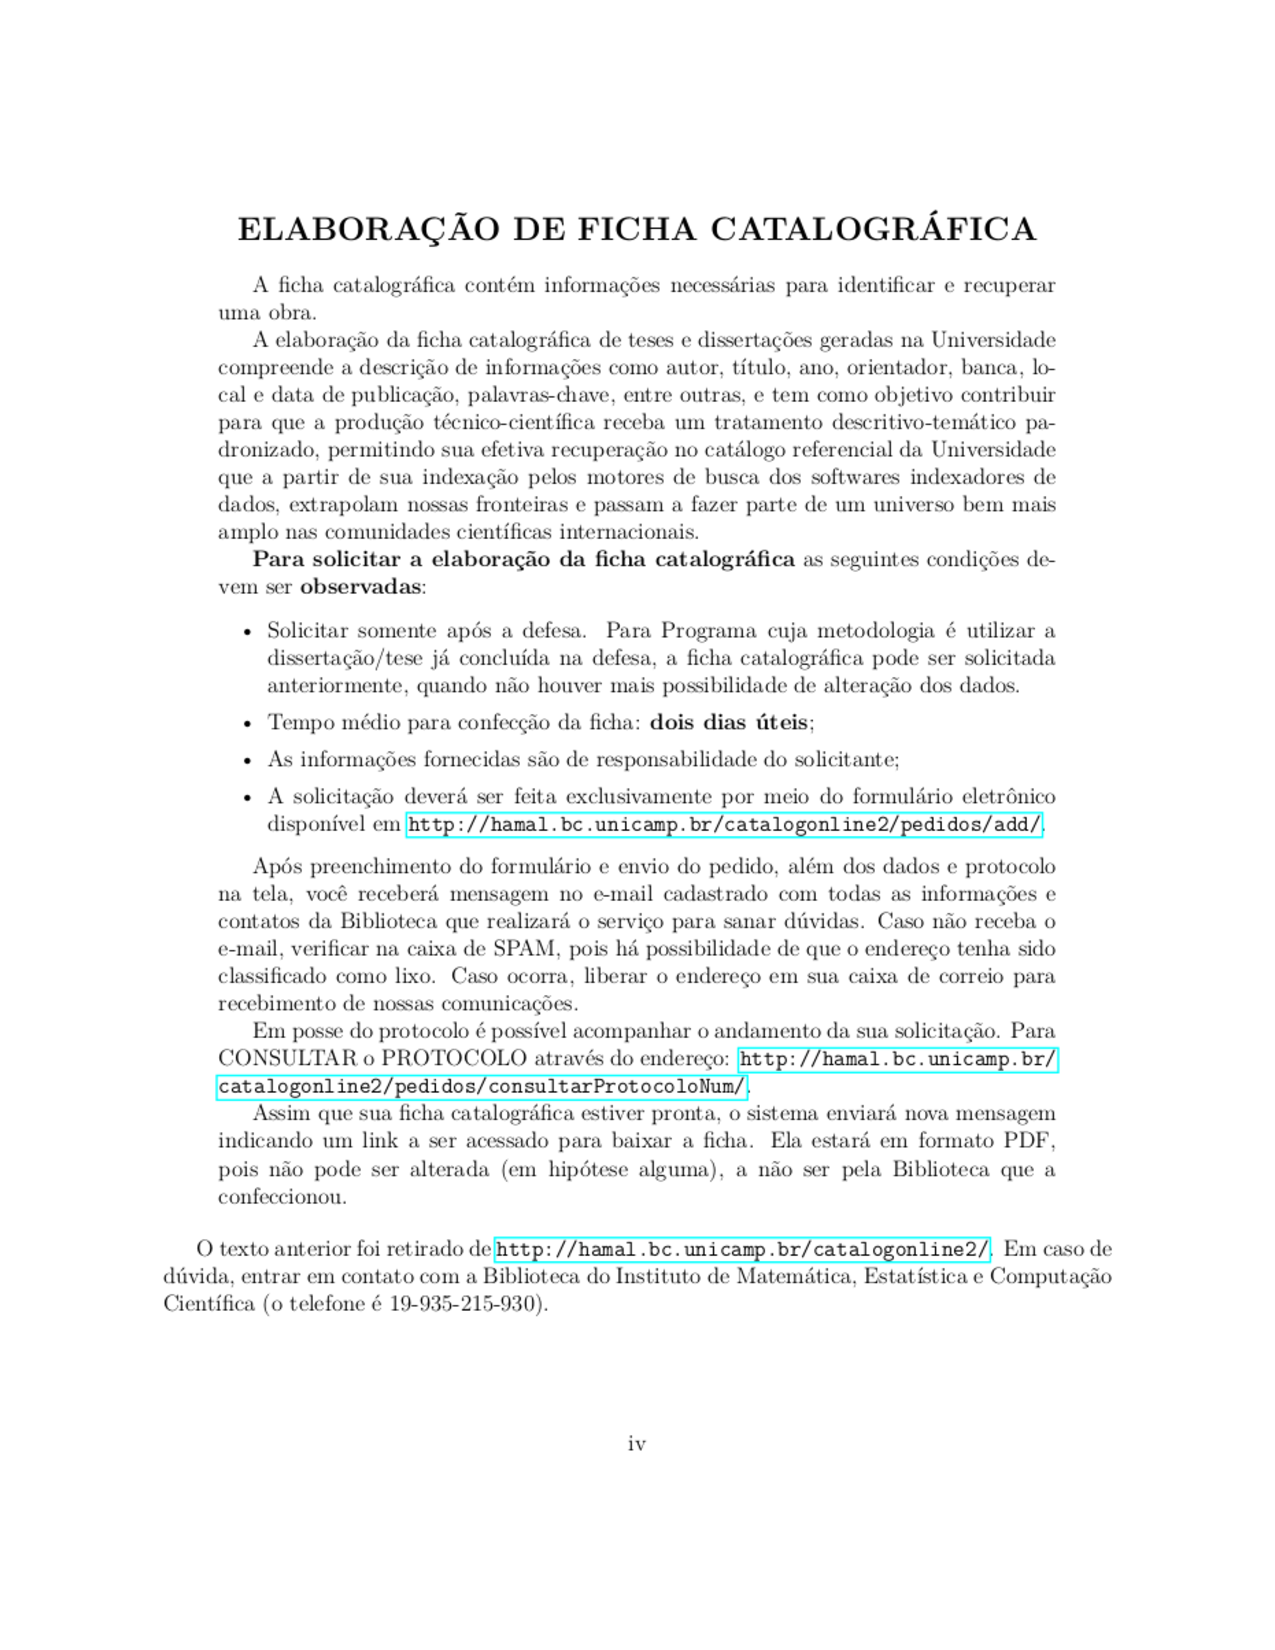
\includepdf{ficha-catalografica}
%
% WARNING A folha de aprovação deve ser assinada pelos membros da banca apos a
% defesa.
% FIXME Substitua o arquivo folha-de-aprovacao.pdf por uma copia escaneada.
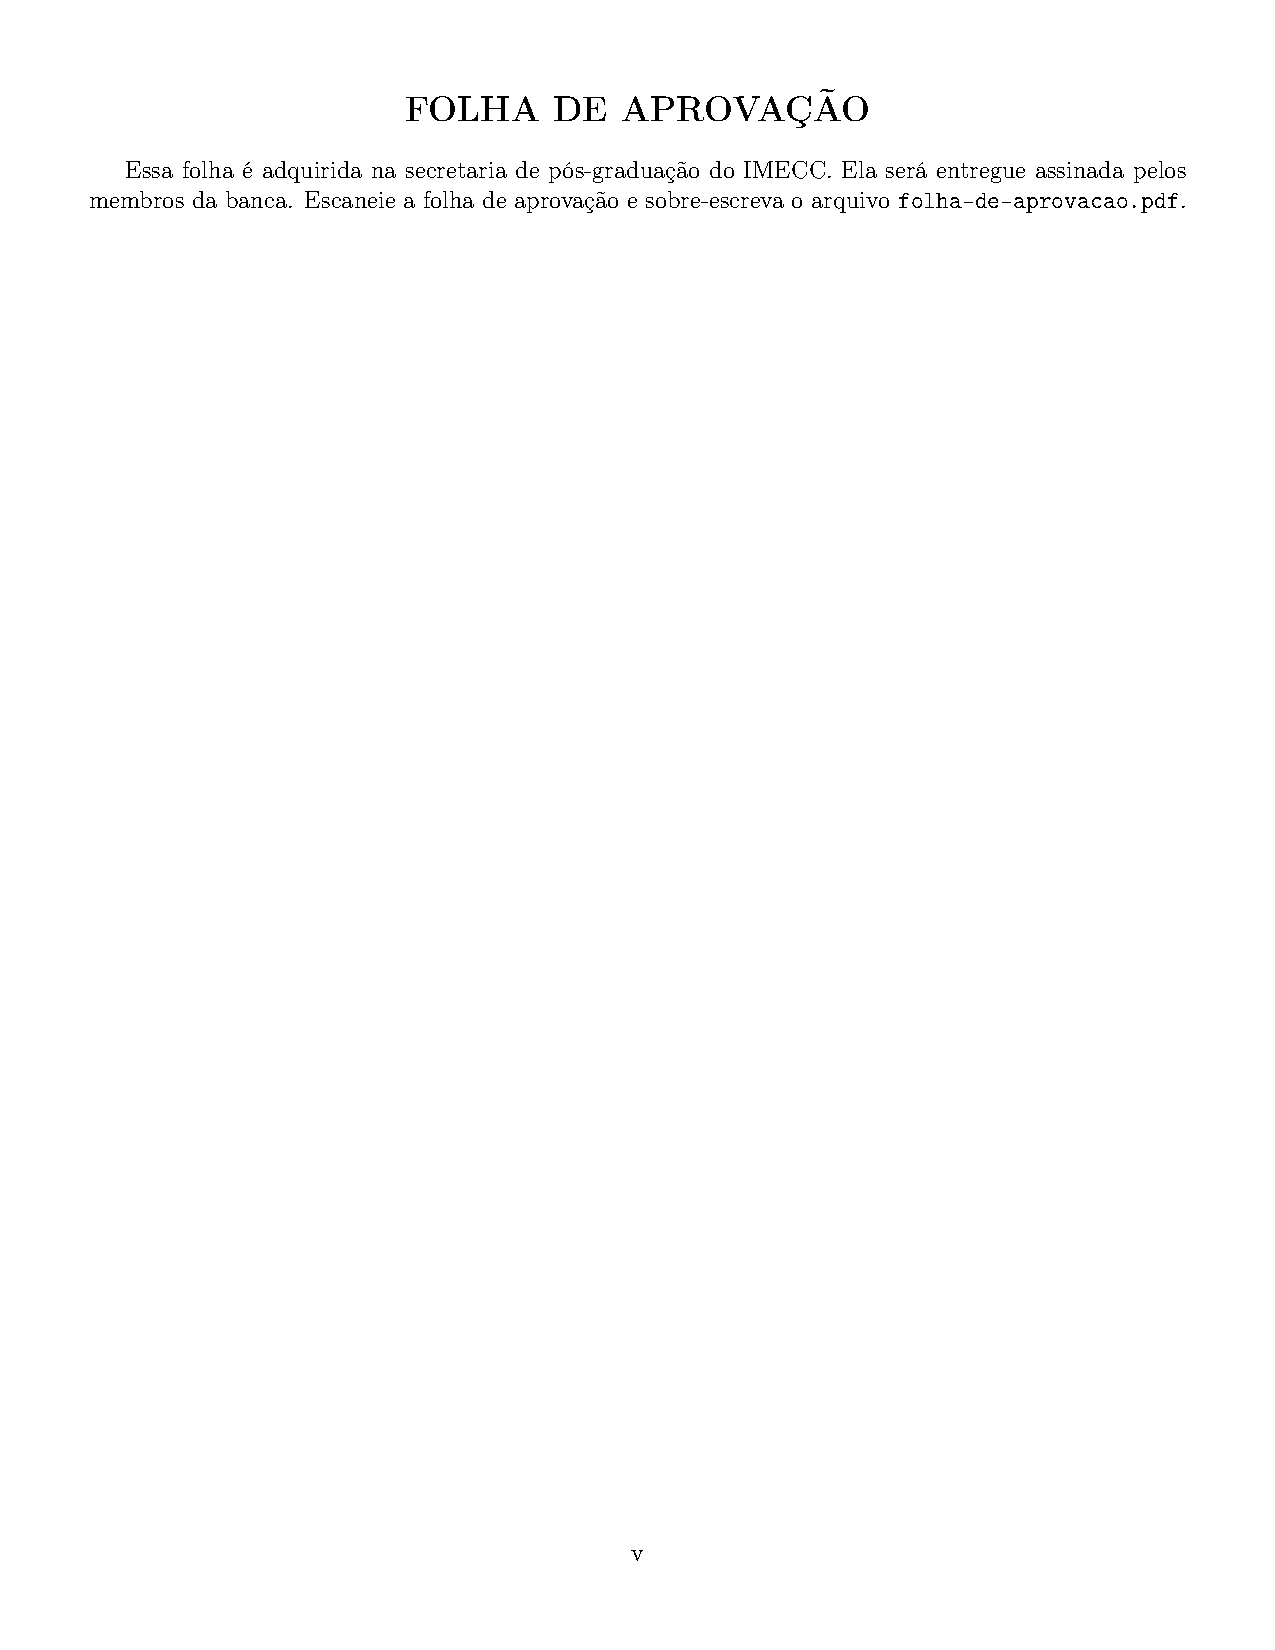
\includepdf{folha-de-aprovacao}
\chapter*{}  % Capítulo vazio.
\begin{center}
  \large{\textbf{Abstract}}
\end{center}

\selectlanguage{english}
% FIXME Delete lines from this one until 14th.
This is the abstract. It must be no longer than 500 words. One easy way to get
a closer number of the words is using:
\begin{lstlisting}
$ detex -l abstract.tex | wc -l
\end{lstlisting}

The keywords that can be used are listed in
\href{http://acervus.unicamp.br/}{Base Acervus}.
% TODO Inserir o resumo em inglês aqui.

\vspace{.5cm}
\textbf{Keywords}:
% FIXME Remover a linha abaixo.
keyword01, keyword02, keyword03.
% TODO Inserir as palavras-chave em inglês aqui.
\selectlanguage{brazilian}
\vspace{.1\textheight}
\begin{center}
  \large{\textbf{Resumo}}
\end{center}

% FIXME Remover deste ponto até a linha 14.
Esse é o resumo. Ele não deve conter mais de 500 palavras. Uma maneira
fácil de obter uma boa aproximação do número de palavras do seu resumo é:
\begin{lstlisting}
$ detex -l resumo.tex | wc -l
\end{lstlisting}

As palavras chaves permitidas podem ser consultadas na
\href{http://acervus.unicamp.br/}{Base Acervus}, buscando pelo campo
\emph{Assunto}.
% TODO Inserir o resumo em português aqui.

\vspace{.2cm}
\textbf{Palavras-chave}:
% FIXME Remover a linha abaixo.
palavra01, palavra02, palavra03.
% TODO Inserir as palavras-chave aqui.
%
\tableofcontents
%
% FIXME Se não for incluir a dedicatória, comentar a linha abaixo.
\chapter*{\markboth{}{}}  % \markboth{}{} é utilizado para corrigir o cabeçalho.
\phantomsection
\addcontentsline{toc}{chapter}{Dedicatória}
\begin{center}
  \emph{
  % FIXME Remover as duas linhas abaixo.
  Aos meus \ldots. \\
  Para \ldots.} 
  % TODO Inserir a dedicatória aqui.
\end{center}
%
% FIXME Se não for incluir os agradecimentos, comentar a linha abaixo.
\chapter*{Agradecimentos\markboth{Agradecimentos}{}}  % \markboth{}{} é utilizado para corrigir o cabeçalho.
\phantomsection
\addcontentsline{toc}{chapter}{Agradecimentos}
% FIXME Escrever os agradecimentos.
Aqui deve-se agradecer quem merece agradecimento

Se recebeu bolsa de algum órgão de fomento, não esqueça de agradecê-lo.
%
% FIXME Comentar a linha abaixo se não desejar listar as figuras
% apresentadas.
\renewcommand{\listfigurename}{Lista de Ilustrações}  % CCPG 228/2013
\listoffigures
%
% FIXME Comentar a linha abaixo se não desejar listar as tabelas
% apresentadas.
\listoftables
%
% FIXME Comentar a linha abaixo de não for apresentar as
% abreviações e siglas utilizadas.
\chapter*{Lista de Abreviaturas e Siglas\markboth{Lista de Abreviaturas e Siglas}{}}  % \markboth{}{} é utilizado para corrigir o cabeçalho.

\begin{description}
  % FIXME Remover as duas abreviações/siglas abaixo e incluir as que serão
  % utilizadas.
  \item[FIXME] Indica que algo deve ser consertado.
  \item[TODO] Indica que algo deve ser feito.
\end{description}
%
% FIXME Comentar a linha abaixo se não for apresentar os
% símbolos utilizados.
\chapter*{Lista de Símbolos\markboth{Lista de Símbolos}{}}  % \markboth{}{} é utilizado para corrigir o cabeçalho.

\begin{description}
    % FIXME Remover os dois símbolos abaixo e incluir as que serão
    % utilizadas.
    \item[$\diamond$] Representa um diamante.
    \item[$\lhd$] Representa um deslocamento para a esquerda.
    \item[$\rhd$] Representa um deslocamento para a direita.
\end{description}
%
% FIXME Comentar a linha abaixo se não desejar listar os algoritmos
% apresentados.
\listofalgorithms
%
% FIXME Comentar a linha abaixo se não desejar listar os trechos de código
% apresentados.
\lstlistoflistings
%
% As paginas com o conteúdo da tese são numeradas com algoritmos arábicos.
\mainmatter
%
% FIXME Remover as 3 linhas abaixo.
\chapter{Título 1}
Esse é o primeiro capítulo da sua tese.

\section{Seção 1.1}
Essa é uma seção da sua tese.

\subsection{Subseção 1.1.1}

Essa é uma subseção da sua tese.

\subsection{Subseção 1.1.2}

Essa é outra subseção da sua tese.

\section{Equações matemáticas}
Para equações matemáticas está sendo utilizado os seguintes
pacotes:
\begin{itemize}
  \item amsmath,
  \item amsfonts,
  \item amssymb,
  \item amsthm,
  \item breqn.
\end{itemize}

Um exemplo de equação na mesma linha: 
$ 1 + 1 + 1 + 1 + 1 + 1 = 6$, 
que é trivial\index{trivial} de ser verificada.

Equações na mesma linha são quebradas automaticamente:
$ 1 + 1 + 1 + 1 + 1 + 1 + 1 + 1 + 1 + 1 + 1 + 1 = 12$. 

Ao utilizar equações na mesma linha deve-se tomar o cuidado de manter a
legibilidade da equação e não modificar a altura da linha. É
errado utilizar $\frac{1}{2} + \frac{1}{2} = 1$ ou $\frac{\partial}{\partial x}
(y^2 + 2xy + x^2) = 2y + 2x$, devendo ser utilizado $(1/2) + (1/2) = 1$ ou
$\partial (y^2 + 2 x y + x^2) / \partial x = 2 y + 2 x$.

Além de equações na mesma linha, também é possível
utilizar equações em destaque:
\begin{equation}
  1 + 1 + 1 + 1 + 1 + 1 = 6
\end{equation}
ou
\begin{equation*}
  1 + 1 + 1 + 1 + 1 + 1 = 6.
\end{equation*}
Ao utilizar equações matemáticas em destaque, não esqueça da pontuação nas
equações.

Recomenda-se utilizar os ambientes
\begin{itemize}
  \item dmath(*) e
  \item dgroup(*)
\end{itemize}
disponibilizados pelo pacote breqn ao invés dos ambientes
\begin{itemize}
  \item equation(*,)
  \item align(*),
  \item multiline(*) e
  \item split
\end{itemize}
pois os primeiros quebram e alinham automaticamente as equações em destaque.
Veja a seguir a ``equivalência'' entre os ambientes:
\begin{description}
  \item[dmath]
    \begin{dmath}
      1 + 1 + 1 + 1 + 1 + 1 + 1 + 1 + 1 + 1 + 1 + 1 + 1 + 1 + 1 + 1 + 1 + 1 + 1
      + 1 + 1 + 1 + 1 + 1 + 1 + 1 + 1 + 1 + 1 + 1 = 30
    \end{dmath}
  \item[equation] 
    \begin{equation}
      1 + 1 + 1 + 1 + 1 + 1 + 1 + 1 + 1 + 1 + 1 + 1 + 1 + 1 + 1 + 1 + 1 + 1 + 1
      + 1 + 1 + 1 + 1 + 1 + 1 + 1 + 1 + 1 + 1 + 1 = 30
    \end{equation}
  \item[equation com split] 
    \begin{equation}
      \begin{split}
        1 + 1 + 1 + 1 + 1 + 1 + 1 + 1 + 1 + 1 + 1 + 1 + 1 + 1 + 1 \\
        + 1 + 1 + 1 + 1 + 1 + 1 + 1 + 1 + 1 + 1 + 1 + 1 + 1 + 1 + 1 = 30 
      \end{split}
    \end{equation}
  \item[align] 
    \begin{align}
      1 + 1 + 1 + 1 + 1 + 1 + 1 + 1 + 1 + 1 + 1 + 1 + 1 + 1 + 1 \\
      + 1 + 1 + 1 + 1 + 1 + 1 + 1 + 1 + 1 + 1 + 1 + 1 + 1 + 1 + 1 = 30 
    \end{align}
  \item[align com quebra de linha] 
    \begin{align}
      1 + 1 + 1 + 1 + 1 + 1 + 1 + 1 + 1 + 1 + 1 + 1 + 1 + 1 + 1 \\
      + 1 + 1 + 1 + 1 + 1 + 1 + 1 + 1 + 1 + 1 + 1 + 1 + 1 + 1 + 1 = 30 
    \end{align}
\end{description}

No caso do desenvolvimento/simplificação de uma expressão
matemática também é recomendado utilizar os ambientes
disponibilizados pelo pacote breqn.
\begin{description}
  \item[dmath]
    \begin{dmath}
      f(x) = 1 + 1 + 1 + 1 + 1 + 1 + 1 + 1 + 1 + 1 + 1 + 1 + 1 + 1 + 1 + 1 + 1 +
      1 + 1 + 1 + 1 + 1 + 1 + 1 + 1 + 1 + 1 + 1 + 1 + 1
      = 2 + 2 + 2 + 2 + 2 + 2 + 2 + 2 + 2 + 2 + 2 + 2 + 2 + 2 + 2
      = 4 + 4 + 4 + 4 + 4 + 4 + 4 + 2
      = 8 + 8 + 8 + 6
      = 16 + 14
      = 30
    \end{dmath}
  \item[equation com split] 
    \begin{equation}
      \begin{split}
        f(x) &= 1 + 1 + 1 + 1 + 1 + 1 + 1 + 1 + 1 + 1 + 1 + 1 + 1 + 1 + 1 + 1 + 1 \\
        &\quad {}+ 1 + 1 + 1 + 1 + 1 + 1 + 1 + 1 + 1 + 1 + 1 + 1 + 1 \\
        &= 2 + 2 + 2 + 2 + 2 + 2 + 2 + 2 + 2 + 2 + 2 + 2 + 2 + 2 + 2 \\
        &= 4 + 4 + 4 + 4 + 4 + 4 + 4 + 2 \\
        &= 8 + 8 + 8 + 6 \\
        &= 16 + 14 \\
        &= 30
      \end{split}
    \end{equation}
  \item[align com quebra de linha] 
    \begin{align}
        f(x) &= 1 + 1 + 1 + 1 + 1 + 1 + 1 + 1 + 1 + 1 + 1 + 1 + 1 + 1 + 1 + 1 + 1 \\
        &\quad {}+ 1 + 1 + 1 + 1 + 1 + 1 + 1 + 1 + 1 + 1 + 1 + 1 + 1 \\
        &= 2 + 2 + 2 + 2 + 2 + 2 + 2 + 2 + 2 + 2 + 2 + 2 + 2 + 2 + 2 \\
        &= 4 + 4 + 4 + 4 + 4 + 4 + 4 + 2 \\
        &= 8 + 8 + 8 + 6 \\
        &= 16 + 14 \\
        &= 30
    \end{align}
\end{description}

Para o caso de equações relacionadas e que devem ser agrupadas,
temos
\begin{description}
  \item[dgroup com dmath]
    \begin{dgroup}
      \begin{dmath}
        f(x) = 1 + 1 + 1 + 1 + 1 + 1 + 1 + 1 + 1 + 1 + 1 + 1 + 1 + 1 + 1 + 1 + 1
        + 1 + 1 + 1 + 1 + 1 + 1 + 1 + 1 + 1 + 1 + 1 + 1 + 1
        = 2 + 2 + 2 + 2 + 2 + 2 + 2 + 2 + 2 + 2 + 2 + 2 + 2 + 2 + 2
        = 4 + 4 + 4 + 4 + 4 + 4 + 4 + 2
        = 8 + 8 + 8 + 6
        = 16 + 14
        = 30
      \end{dmath}
      \begin{dmath}
        g(x) = 2 + 2 + 2 + 2
        = 4 + 4
        = 8
      \end{dmath}
    \end{dgroup}
  \item[subequations com equation com split] 
    \begin{subequations}
      \begin{equation}
        \begin{split}
          f(x) &= 1 + 1 + 1 + 1 + 1 + 1 + 1 + 1 + 1 + 1 + 1 + 1 + 1 + 1 + 1 + 1 + 1 \\
          &\quad {}+ 1 + 1 + 1 + 1 + 1 + 1 + 1 + 1 + 1 + 1 + 1 + 1 + 1 \\
          &= 2 + 2 + 2 + 2 + 2 + 2 + 2 + 2 + 2 + 2 + 2 + 2 + 2 + 2 + 2 \\
          &= 4 + 4 + 4 + 4 + 4 + 4 + 4 + 2 \\
          &= 8 + 8 + 8 + 6 \\
          &= 16 + 14 \\
          &= 30
        \end{split}
      \end{equation}
      \begin{equation}
        \begin{split}
          g(x) &= 2 + 2 + 2 + 2 \\
          &= 4 + 4 \\
          &= 8
        \end{split}
      \end{equation}
    \end{subequations}
  \item[align com split] 
    \begin{align}
      \begin{split}
        f(x) &= 1 + 1 + 1 + 1 + 1 + 1 + 1 + 1 + 1 + 1 + 1 + 1 + 1 + 1 + 1 + 1 + 1 \\
        &\quad {}+ 1 + 1 + 1 + 1 + 1 + 1 + 1 + 1 + 1 + 1 + 1 + 1 + 1 \\
        &= 2 + 2 + 2 + 2 + 2 + 2 + 2 + 2 + 2 + 2 + 2 + 2 + 2 + 2 + 2 \\
        &= 4 + 4 + 4 + 4 + 4 + 4 + 4 + 2 \\
        &= 8 + 8 + 8 + 6 \\
        &= 16 + 14 \\
        &= 30
      \end{split} \\
      \begin{split}
        g(x) &= 2 + 2 + 2 + 2 \\
        &= 4 + 4 \\
        &= 8
      \end{split}
    \end{align}
\end{description}

\subsection{Referência cruzada}
Parte das equações anteriores encontram-se numeradas. Esse número pode ser
facilmente acessado se junto da equação tiver sido utilizando o comando label:
\begin{dmath}
  c^2 = a^2 + b^2. \label{eq:exem_pitagoras}
\end{dmath}
E para acessar o número utiliza o comando eqref, \eqref{eq:exem_pitagoras}.

Além de numerar equações também é possível nomeá-las utilizando o comando
tag\footnote{O pacote breqn não possue suporte ao comando tag.}:
\begin{align}
  c^2 &= a^2 + b^2 - 2 a b \cos\theta 
  \label{eq:exem_pitagoras_generalizado}
  \tag{GTP}
\end{align}
E para acessar o nome utiliza-se o comando eqref,
\eqref{eq:exem_pitagoras_generalizado}.

Para que no pdf não apareça o parâmetro dos comandos label é preciso remover o
pacote showlabels do arquivo pacotes.tex.

\section{Definições}
Vários ambientes já estão definidos como: Teorema, Conjectura, Corolário,
Definição, \ldots

\begin{thm}
  Teorema, Teorema, Teorema, Teorema.
\end{thm}
\begin{proof}
  Demostração do Teorema.
\end{proof}

\begin{con}
  Conjectura, Conjecture, Conjectura, Conjectura.
\end{con}
\begin{proof}
  Demostração do Conjectura.
\end{proof}

\begin{cor}
  Corolário, Corolário, Corolário, Corolário.
\end{cor}
\begin{proof}
  Demostração do Corolário.
\end{proof}

\begin{dfn}
  Definição, Definição, Definição.
\end{dfn}
\begin{proof}
  Demostração da Definição.
\end{proof}

Use esses ambientes de maneira sábia.
\chapter{Título 2}
Esse é o segundo capítulo da sua defesa.

\section{Figuras}
É possível inserir figuras na sua defesa utilizando o comando
\lstinline+\includegraphics{caminho_figura}+. \\

\includegraphics[width=0.1\textwidth]{figuras/unicamp-logo}

É recomendado deixar as figuras\index{figura} como objetos flutuantes, para isso
utiliza-se o ambiente \lstinline+figure+.
\begin{figure}[!htb]
  \center
  
\includegraphics[width=0.1\textwidth]{figuras/unicamp-logo}
  \caption{Logo da UNICAMP.}
  \label{fig:log_unicamp}
\end{figure}

Além de inserir figuras é possível ``desenhar''\index{figura!desenhar} figuras
utilizando o pacote TikZ\index{figura!TikZ}, como na
Figura~\ref{fig:exem_tikz1}~e~\ref{fig:exem_tikz2}.
\begin{figure}[!htb]
  \centering
  \begin{tikzpicture}
    \draw (0,0) -- (0,2) -- (2,2) -- (2,0) -- (0,0);
    \fill (5,0) circle (1);
  \end{tikzpicture}
  \caption{Exemplo do uso do TikZ.}
  \label{fig:exem_tikz1}
\end{figure}
\begin{figure}[!htb]
  \centering
  \begin{tikzpicture}
    \node[draw] (A) at (0,1) {$A$};
    \node[draw,circle] (B) at (0,-1) {$B$};
    \node (C) at (1,0) {$C$};
    \node[fill=red,text=black] (D) at (3,0) {$D$};
    \node[draw,rectangle,fit=(A) (B) (C)] {};

    \draw[->] (A) -- (D);
    \draw[->] (B) -- (D);
    \draw[->] (C) -- (D);

    \coordinate (a) at (5,1);
    \coordinate (b) at (5,-1);

    \draw[dashed] (D) -- (a);
    \draw[dotted] (D) -- (b);
    \draw[<->] (a) -- (b);
  \end{tikzpicture}
  \caption{Outro exemplo do uso do TikZ.}
  \label{fig:exem_tikz2}
\end{figure}

\section{Tabelas}
Além de figuras também é possível inserir tabelas utilizando o ambiente
\lstinline+tabular+. \\
\begin{tabular}{cc}
  \toprule
  Tabela & Tabela \\
  \midrule
  Tabela & Tabela \\
  \bottomrule
\end{tabular}

Assim como as figuras, é recomendado que as tabelas sejam incluídas como
objetos flutuantes, para isso utiliza-se o ambiente \lstinline+table+.
\begin{table}[!htb]
  \caption{Exemplo de Tabela.}
  \label{tab:exem}
  \centering
  \begin{tabular}{cc}
    \toprule
    Tabela & Tabela \\
    \midrule
    Tabela & Tabela \\
    \bottomrule
  \end{tabular}
\end{table}

Além de inserir tabelas manualmente, como na Tabela~\ref{tab:exem}, também é
possível utilizar arquivos \emph{.csv} para criar tabelas. Neste caso, é
necessário incluir o pacote \texttt{csvsimple} que não foi incluído por questão
de compatibilidade com distribuições do \LaTeX \ anteriores a 2009.
\chapter{Título 3}
Esse é o terceiro capítulo da sua tese.

\section{Algoritmos}
Para facilitar a leitura, é bom incluir o algoritmo\index{algoritmo} de forma
adequada e não como uma lista, para isso utilize o ambiente
\lstinline+algorithmic+.
\begin{algorithmic}[2]
  \STATE $i \leftarrow 0$
  \STATE $y \leftarrow 0$
  \FOR{$i \leq 10$}
    \STATE $y \leftarrow y + i$
    \STATE $i \leftarrow i + 1$
  \ENDFOR
\end{algorithmic}

É possível nomear os algoritmos\index{algoritmo} ao utilizar o ambiente
\lstinline+algorithm+.
\begin{algorithm}
  \caption{Loop infinito.}
  \label{alg:loop_inf}
  \begin{algorithmic}
    \REQUIRE $n \geq 0$
    \ENSURE $y = 1 + 2 + \ldots + n$
    \STATE $y \leftarrow 0$
    \STATE $i \leftarrow 0$
    \IF{$n < 0$}
      \PRINT Entrada inadequada.
    \ELSE
      \WHILE{$i \neq n$}
        \STATE $y \leftarrow y + i$
      \ENDWHILE
    \ENDIF
  \end{algorithmic}
\end{algorithm}

Recomenda-se traduzir as instruções utilizadas no algoritmo. Para isso, é
preciso dar uma olhada na documentação do pacote \lstinline+algorithmic+.

\section{Códigos}
Em alguns casos, recomenda-se incluir um trecho de
código\index{codigo@código} e para isso utiliza-se o comando
\lstinline+\lstinputlisting{codigo}+.
\lstinputlisting[firstline=5, lastline=5, nolol=true]{src/exem.c}

Assim como os algoritmos também é possível nomear os códigos.
\lstinputlisting[firstline=10, lastline=12, caption=Loop em C,
language=C,  frame=single]{src/exem.c}
\chapter{Título 4}
Esse é o terceiro capítulo da sua tese.

\section{Referência bibliográfica}
Para a referência bibliográfica é utilizado o BibTeX e o pacote
\lstinline+biblatex+. Poderia ser utilizado apenas o BibTeX mas existem algumas
funcionalidades disponibilizadas no pacote \lstinline+biblatex+ que são muito
convenientes.

\subsection{BibTeX}
BibTeX é o nome de um formato de ``banco de dados'' para referências
bibliográficas desenvolvido para ser utilizado em conjunto com o LaTeX e também
do programa responsável por processar esse ``banco de dados''.

O ``banco de dados'' corresponde a um arquivo de texto com a extensão
\lstinline+.bib+ e cada referência no BibTeX segue a seguinte estrutura:
\begin{lstlisting}
@TIPO_DOCUMENTO{identificador,
campo1 = {valor do campo 1},
campo2 = {valor do campo 2},
campo3 = {valor do campo 3},
...
}
\end{lstlisting}

Para saber quais os \lstinline+TIPO_DOCUMENTO+ existentes e sobre os
campos recomenda-se a documentação do BibTeX que pode ser acessada pelo comando:
\begin{lstlisting}
$ texdoc bibtex
\end{lstlisting}

Uma das grandes vantagens de se utilizar o BibTeX é que as chances de encontrar
o BibTeX de algum material na internet é extremamente alta. Tanto o Google
Scholar como o Google Books disponibilizam o BibTeX para todos os materiais
indexados em suas respectivas bases de dados.

Por padrão este modelo\nocite{ModeloIMECC} utiliza o arquivo
\lstinline+tese.bib+ que inicialmente possue apenas a referência deste modelo:
\begin{lstlisting}
@Misc{ModeloIMECC,
    author = {Raniere Silva and Tiago Macedo and Junior Soares
    and others},
    title = {Modelo de Dissertacao/Tese do Instituto de
Matematica, Estatistica e Computacao Cientifica ({IMECC}) da
Universidade Estadual de Campinas ({UNICAMP})},
    year = {2013},
    url = {https://github.com/r-gaia-cs/modelo_tese_imecc},
}
\end{lstlisting}

Se desejar adicionar mais arquivos com a extensão \lstinline+.bib+, adicione no
arquivo \lstinline+configuracoes.tex+ uma linha semelhante a
\begin{lstlisting}
\addbibresource{seu_arquivo.bib}
\end{lstlisting}

Se nunca tiver utilizado o BibTeX e desejar mais exemplos de como escrever sua
referência no arquivo \lstinline+.bib+ pois não encontrou-a disponível na
internet, você pode dar uma olhada no arquivo
\lstinline+biblatex_style_samples/sample.bib+ presente neste modelo.

\subsection{\lstinline+biblatex+}
Para que uma entrada do \lstinline+tese.bib+ seja incluído na referência
bibliográfica ele precisa ser utilizado em algum dos arquivos \lstinline+.tex+
que compõe sua dissertação/tese. Para utilizar uma referência utiliza-se uma das
variantes do comando \lstinline+\cite{id}+, onde
\lstinline+id+ correspode ao \lstinline+identificador+ utilizado na entrada do
BibTeX para a referência desejada.

O comando \lstinline+\cite{id}+ insere o número da referência entre colchetes,
como mostrado abaixo:
\begin{table}[!h]
  \centering
  \begin{tabular}{lc}
    \toprule
    Comando & Resultado \\ \midrule
    \lstinline+\cite{Swa82}+ & \cite{Swa82} \\
    \lstinline+\cite{Bailey}+ & \cite{Bailey} \\
    \lstinline+\cite{Ta}+ & \cite{Ta} \\
    \lstinline+\cite{Hale}+ & \cite{Hale} \\ \bottomrule
  \end{tabular}
\end{table}

Para inserir o nome dos autores e o número da referência entre colchetes,
utiliza-se o comando \lstinline+\textcite{id}+, como mostrado abaixo:
\begin{table}[!h]
  \centering
  \begin{tabular}{ll}
    \toprule
    Comando & Resultado \\ \midrule
    \lstinline+\textcite{Swa82}+ & \textcite{Swa82} \\
    \lstinline+\textcite{Bailey}+ & \textcite{Bailey} \\
    \lstinline+\textcite{Ta}+ & \textcite{Ta} \\
    \lstinline+\textcite{Hale}+ & \textcite{Hale} \\ \bottomrule
  \end{tabular}
\end{table}

Para inserir apenas o nome dos autores utiliza-se o comando
\lstinline+\citeauthor{id}+, como mostrado abaixo:
\begin{table}[!h]
  \centering
  \begin{tabular}{ll}
    \toprule
    Comando & Resultado \\ \midrule
    \lstinline+\citeauthor{Swa82}+ & \citeauthor{Swa82} \\
    \lstinline+\citeauthor{Bailey}+ & \citeauthor{Bailey} \\
    \lstinline+\citeauthor{Ta}+ & \citeauthor{Ta} \\
    \lstinline+\citeauthor{Hale}+ & \citeauthor{Hale} \\ \bottomrule
  \end{tabular}
\end{table}

Para inserir apenas o título da referência utiliza-se o comando
\lstinline+\citetitle{id}+, como mostrado abaixo:
\begin{table}[!h]
  \centering
  \begin{tabular}{ll}
    \toprule
    Comando & Resultado \\ \midrule
    \lstinline+\citetitle{Swa82}+ & \citetitle{Swa82} \\
    \lstinline+\citetitle{Bailey}+ & \citetitle{Bailey} \\
    \lstinline+\citetitle{Ta}+ & \citetitle{Ta} \\
    \lstinline+\citetitle{Hale}+ & \citetitle{Hale} \\ \bottomrule
  \end{tabular}
\end{table}

Para inserir apenas o ano de publicação da referência utiliza-se o comando
\lstinline+\citeyear{id}+, como mostrado abaixo:
\begin{table}[!h]
  \centering
  \begin{tabular}{lc}
    \toprule
    Comando & Resultado \\ \midrule
    \lstinline+\citeyear{Swa82}+ & \citeyear{Swa82} \\
    \lstinline+\citeyear{Bailey}+ & \citeyear{Bailey} \\
    \lstinline+\citeyear{Ta}+ & \citeyear{Ta} \\
    \lstinline+\citeyear{Hale}+ & \citeyear{Hale} \\ \bottomrule
  \end{tabular}
\end{table}

Para citações múltiplas, utiliza-se os comandos \lstinline+\cites{id1,id2,id3}+
ou \lstinline+\textcites{id1,id2,id3}+, como mostrado abaixo:
\begin{table}[!h]
  \centering
  \begin{tabular}{lc}
    \toprule
    Comando & Resultado \\ \midrule
    \lstinline+\cites{Bailey,Swa82}+ & \cites{Bailey,Swa82} \\
    \lstinline+\cites{Hale,Ta}+ & \cites{Hale,Ta} \\
    \lstinline+\textcites{Bailey,Swa82}+ & \textcites{Bailey,Swa82} \\
    \lstinline+\textcites{Hale,Ta}+ & \textcites{Hale,Ta} \\ \bottomrule
  \end{tabular}
\end{table}

Caso deseje incluir uma referência na referência bibliográfica mas
suprimí-la ao longo do texto você deve utilizar o comando
\lstinline+\nocite{id}+.

Por último, caso deseje incluir todas as referências presentes no arquivo
\lstinline+.bib+, você pode utilizar o comando \lstinline+\nocite{*}+.\nocite{*}

\section{Estilos}
O pacote \lstinline+biblatex+ oferece vários estilos por padrão, sendo alguns
deles são:
\begin{itemize}
  \item \lstinline+numeric+,
  \item \lstinline+alphabetic+,
  \item \lstinline+authoryear+,
  \item \lstinline+authortitle+,
  \item \lstinline+verbose+.
\end{itemize}

O estilo padrão deste modelo é o estilo padrão do \lstinline+biblatex+ que
corresponde ao \lstinline+numeric+. Se você desejar utilizar um outro estilo
cujo nome é \lstinline+estilo_desejado+ você precisa trocar a linha
\begin{lstlisting}
\usepackage{biblatex}
\end{lstlisting}
no arquivo \lstinline+pacotes.tex+ por
\begin{lstlisting}
\usepackage[style=estilo_desejado]{biblatex}
\end{lstlisting}

Para facilitar sua vida, no diretório \lstinline+biblatex_style_samples+ você
encontrará alguns PDFs ilustrando alguns dos estilos disponibilizados pelo
\lstinline+biblatex+. Esses arquivos PDFs encontram-se ilustrados no
Apêndice~\ref{ape:estilo_biblatex}.

Se nenhum dos estilos oferecidos lhe agradar você poderá escrever seu próprio
estilo, mas para isso terá que ler a documentação do \lstinline+biblatex+.
%
% TODO Inserir os arquivos referentes ao corpo da tese.
%
% Referência bibliográfica.
\cleardoublepage
\phantomsection
\addcontentsline{toc}{chapter}{Referências}
\printbibliography[title=Referências]
%
% FIXME Se não for utilizar apêndices (o glossario é um apêndice), comentar a
% linha abaixo.
\appendix
% FIXME Remover as 4 linha abaixo.
\chapter*{Glossário\markboth{Glossário}{}}  % \markboth{}{} é utilizado para corrigir o cabeçalho.
\addcontentsline{toc}{chapter}{Glossário}

\begin{description}
  % FIXME Remover as duas explicações abaixo e incluir as que serão
  % utilizadas.
  \item[Tese] Proposição que é enunciada e sustentada.
  \item[Dissertação] Discurso, exposição ou exame minucioso de
    determinado assunto.
\end{description}
\chapter{Título do Apêndice}
Esse é um apêndice da sua tese.

Como informado no ``Manual de Normalização para o NITEG e o PPGCI da ECI-UFMG''
disponível em
\url{http://ppgci.eci.ufmg.br/normalizacao/?Reda%E7%E3o_e_Estilo:Anexo_e_ap%EAndice}:
\begin{quote}
  Apêndices são os materiais elaborados pelo próprio autor com objetivo de
  completar uma argumentação. 
\end{quote}

\section{Seção A.1}
Essa é uma seção de um dos apêndices da sua tese.
\chapter{Git}
Git é o atual \textit{state-of-the-art} sistema de controle de versão e tem sido
utilizado em vários projetos, muitos na área de desenvolvimento de software,
sendo o grande destaque o Kernel Linux. Este modelo de tese possui suas versões
controladas por meio do Git e na próxima sessão será apresentado algumas
dicas de como utilizar o Git para aproveitar melhor este modelo por meio da
linha de comando e na sessão seguinte pela interface gráfica nativa do Git.

\section{Pela linha de comando}
\subsection{Baixando o modelo}
Para baixar o modelo utilizando o Git você deve executar o comando:
\begin{lstlisting}[escapechar=@]
$ git clone https://github.com/r@-@gaia@-@cs/modelo_tese_imecc.git
\end{lstlisting}
Será criado uma pasta \lstinline+modelo_tese_imecc+ com os arquivos do
modelo.

Além da versão oficial do modelo existem algumas outras e para ver uma lista
destas versões você deve executrar o comando:
\begin{lstlisting}
$ git branch
\end{lstlisting}
Para selecionar a versões a ser utilizada, execute o comando:
\begin{lstlisting}
$ git branch versao_desejada
\end{lstlisting}
A versão oficial é chamada de \lstinline+master+.

Antes de começar a editar os arquivos, execute os comandos:
\begin{lstlisting}
$ git branch meu_trabalho
$ git checkout meu_trabalho
\end{lstlisting}

\subsection{Editando o modelo}
Evite ao máximo modificar os arquivos originais do modelo pois isso facilitará a
atualização do mesmo como será apresentado na seção seguinte.

Para adicionar novos arquivos ao controle de versão, execute o comando:
\begin{lstlisting}
$ git add novo_arquivo
\end{lstlisting}
E para adicionar modificações nos arquivos previamente adicionados ao controle
de versão, execute o comando:
\begin{lstlisting}[escapechar=@]
$ git add @-@u
\end{lstlisting}

Para criar uma nova versão da sua dissertação/tese, execute o comando:
\begin{lstlisting}[escapechar=@]
$ git commit @-@m 'Breve descricao do que foi feito ate agora.'
\end{lstlisting}

\subsection{Atualizando o modelo}
Como este modelo é um trabalho em progresso e não existe nenhuma garantia de que
as deliberações da Comissão Central de Pós-Graduação serão mantidas até que você
termine seu mestrado/doutorado é importante existir uma maneira de você
atualizar sua dissertação/tese já em processo de escrita com as novas
deliberações.

Antes de você atualizar o modelo, execute o seguinte comando:
\begin{lstlisting}[escapechar=@]
$ git commit @-@m 'Preparacao para atualizacao do modelo.'
\end{lstlisting}
Para atualizar o modelo, execute os comandos:
\begin{lstlisting}
$ git fetch
$ git checkout versao_desejada
$ git merge origin/versao_desejada
$ git checkout meu_trabalho
$ git rebase meu_trabalho versao_desejada
\end{lstlisting}

\section{Pela interface gráfica (git-gui)}
\subsection{Baixando o modelo}
Para baixar o modelo:
\begin{enumerate}
  \item Inicialize o git-gui. Será criada uma janela como a ilustrada abaixo.\\
    \includegraphics[scale=.6]{figuras/git-gui00-0}
  \item Selecione ``Clone Existing Repository'' (ou ``Clonar Repositório
    Existente''). Será criada uma janela como ilustrada abaixo.\\
    \includegraphics[scale=.6]{figuras/git-gui01}\\
  \item Preencha os campos ``Source Location'' (ou ``Endereço de Origem'') e
    ``Target Directory'' (ou ``Endereço de Destino''). O campo ``Source
    Location'' deve possuir exatamente o conteúdo da figura abaixo, i.e.,
    \url{https://github.com/r-gaia-cs/modelo_tese_imecc}, enquanto que ``Target
    Directory'' deve ser uma pasta a sua escolha (sugere-se utilizar o botão
    ``Browse'' ao lado do campo para fazer a seleção da pasta).\\
    \includegraphics[scale=.6]{figuras/git-gui02}
  \item Depois de preencher os campos, pressione o botão ``Clone''. Irá aparecer
    uma janela mostrando o progresso de baixar o modelo e quando terminar
    basta pressione o botão ``Quit''.\\
    \includegraphics[scale=.6]{figuras/git-gui03}
\end{enumerate}

\subsection{Salvando modificações no modelo}
Modifique o modelo utilizando seu editor ou IDE favorito. Depois de realizar
algumas modificações siga os passos abaixo para salvar suas modificações.
\begin{enumerate}
  \item Inicialize o git-gui. Será criada uma janela como a ilustrada abaixo.\\
    \includegraphics[scale=.6]{figuras/git-gui00-1}
  \item Se o endereço de onde salvou o modelo aparecer listado em ``Open Recent
    Repository'' (ou ``Repositórios Abertos Recentemente''), selecione-o. Caso
    contrário pressione ``Open Existing Repository'' (ou ``Abrir Repositório
    Existente'') e selecione a pasta do modelo. Será criada uma janela como a
    ilustrada abaixo.\\
    \includegraphics[scale=.6]{figuras/git-gui04-0}
  \item Partindo da barra de ferramentas no topo da janela, selecione
    \begin{itemize}
      \item \lstinline+Commit -> Rescan+,
      \item \lstinline+Commit -> Stage to Commit+,
      \item \lstinline+Commit -> Stage Changed Files to Commit+.
    \end{itemize}
    A janela terá sido modificada para algo próximo ao ilustrado abaixo.\\
    \includegraphics[scale=.6]{figuras/git-gui05}
  \item Digite um pequeno texto descrevendo as mudanças que fez na caixa de
    texto na parte de baixo da janela como ilustrado abaixo.\\
    \includegraphics[scale=.6]{figuras/git-gui06}
  \item Ao lado da caixa de texto existe um botão ``Commit''. Pressione-o. A
    caixa de texto ficará em branco indicando que as modificações foram
    salvas.\\
    \includegraphics[scale=.6]{figuras/git-gui04-1}
\end{enumerate}

\subsection{Atualizando o modelo}
Como este modelo é um trabalho em progresso e não existe nenhuma garantia de que
as deliberações da Comissão Central de Pós-Graduação serão mantidas até que você
termine seu mestrado/doutorado é importante existir uma maneira de você
atualizar sua dissertação/tese já em processo de escrita com as novas
deliberações.

Uma vez salvo suas modificações como indicado na seção anterior, siga os passos
abaixo:
\begin{enumerate}
  \item Inicialize o git-gui. Será criada uma janela como a ilustrada abaixo.\\
    \includegraphics[scale=.6]{figuras/git-gui00-1}
  \item Se o endereço de onde salvou o modelo aparecer listado em ``Open Recent
    Repository'' (ou ``Repositórios Abertos Recentemente''), selecione-o. Caso
    contrário pressione ``Open Existing Repository'' (ou ``Abrir Repositório
    Existente'') e selecione a pasta do modelo. Será criada uma janela como a
    ilustrada abaixo.\\
    \includegraphics[scale=.6]{figuras/git-gui04-1}
  \item Partindo da barra de ferramentas no topo da janela, selecione
    \lstinline+Remote -> Fetch+ \lstinline+from -> origin+. Irá parecer uma janela
    mostrando o progresso de atualização do modelo. Se ao final do processo de
    atualização a janela for semelhante a\\
    \includegraphics[scale=.6]{figuras/git-gui07-0}\\
    então você pode ignorar os passos a seguir. Já se a janela for semelhante
    a\\
    \includegraphics[scale=.6]{figuras/git-gui07-1}\\
    pressione o botão ``Close'' e prossiga com os passos abaixo.\\
  \item Partindo da barra de ferramentas no topo da janela, selecione
    \lstinline+Merge -> Local Merge+. Irá aparecer uma janela como ilustrada
    abaixo.\\
    \includegraphics[scale=.6]{figuras/git-gui09}
  \item Selecione a opção \lstinline+origin/master+, como ilustrado abaixo, e
    pressione o botão ``Merge''.\\
    \includegraphics[scale=.6]{figuras/git-gui10}
  \item O seu trabalho seja atualizado com base no modelo e o resultado será
    mostrado em uma janela como ilustrado abaixo.\\
    \includegraphics[scale=.6]{figuras/git-gui11}
\end{enumerate}
\chapter{Estilos do biblatex} \label{ape:estilo_biblatex}
Nas páginas a seguir encontram-se exemplos de alguns dos estilos para
referências disponibilizados nativamente pelo pacote \lstinline+biblatex+.
\newpage
\includegraphics[width=1\textwidth]{biblatex_style_samples/numeric} \\
\includegraphics[width=1\textwidth]{biblatex_style_samples/alphabetic} \\
\includegraphics[width=1\textwidth]{biblatex_style_samples/authortitle} \\
\includegraphics[width=1\textwidth]{biblatex_style_samples/verbose} \\
\includegraphics[width=1\textwidth]{biblatex_style_samples/authoryear}
\chapter{Uso de Licenças Creative Commons}
As licenças Creative Commons são uma família de licenças copyleft criada e
mantida pela organização não comercial Creative Commons. Atualmente as licenças
Creative Commons Atribuição 3.0 Não Adaptada (CC-BY) e Creative Commons
Atribuição-CompartilhaIgual 3.0 Não Adaptada (CC-BY-SA) são as licenças mais
utilizadas em conteúdos/recursos abertos.

Os mantenedores deste modelo sugerem a utilizado das licenças CC-BY e CC-BY-SA
por acreditarem que a ciência é melhor desenvolvida quando:
\begin{itemize}
  \item pesquisadores possam compartilhar, utilizar e remixar o trabalho de seus
    colegas (sob a condição de dar os devidos créditos) e
  \item não tenham que se preocupar com a violação de direitos autorais (desde
    que faça atribuição ao autor e trabalho original).
\end{itemize}
Essas são as características de materiais licenciados utilizando CC-BY ou
CC-BY-SA e por isso incentivamos seu uso.

Nas próximas seções você encontrará maiores detalhes sobre as licenças CC-BY e
CC-BY-SA, como utilizá-las em sua dissertação de mestrado ou tese de doutorado e
informações adicionais.

\section{Creative Commons Atribuição 3.0 Não Adaptada}
A licença Creative Commons Atribuição 3.0 Não Adaptada (CC-BY) é a menos restritiva das
licenças Creative Commons. Um material que utiliza essa licença pode ser:
\begin{itemize}
  \item copiado,
  \item distribuído e
  \item modificado
\end{itemize}
por qualquer pessoa desde que indique a obra original e seu autor. Para maiores
informações visite
\url{http://creativecommons.org/licenses/by/3.0/deed.pt_BR}.


Para utilizá-la na sua dissertação de mestrado ou tese de doutorado,
certifique-se do arquivo \lstinline+cc-by.tex+ ter sido incluso no arquivo
\lstinline+tese.tex+ como indicado abaixo:
\begin{lstlisting}
\annex
% TODO Inserir os arquivos referentes aos apendices e anexos.
\chapter{Licença}
Copyright (c) \ano \ de \autor.

Exceto quando indicado o contrário, esta obra está licenciada sob a licença
Creative Commons Atribuição 3.0 Não Adaptada. Para ver uma cópia desta licença,
visite \url{http://creativecommons.org/licenses/by/3.0/}.

\begin{center}
  
\includegraphics{figuras/cc-by.png}
\end{center}

%%%%%%%%%%%%%%%%%%%%%%%%% Exceções da Licença CC-BY-SA %%%%%%%%%%%%%%%%%%%%%%%%%

A marca e o logotipo da UNICAMP são propriedade da Universidade Estadual de
Campinas. Maiores informações sobre encontram-se disponíveis em
\url{http://www.unicamp.br/unicamp/a-unicamp/logotipo/normas%20oficiais-para-uso-do-logotipo}.

\section{Sobre a licença dessa obra}
A licença Creative Commons Atribuição 3.0 Não Adaptada utilizada nessa obra diz
que:
\begin{enumerate}
  \item Você tem a liberdade de:
    \begin{itemize}
      \item Compartilhar — copiar, distribuir e transmitir a obra;
      \item Remixar — criar obras derivadas;
      \item fazer uso comercial da obra.
    \end{itemize}
  \item Sob as seguintes condições:
    \begin{itemize}
      \item Atribuição — Você deve creditar a obra da forma especificada pelo
        autor ou licenciante (mas não de maneira que sugira que estes concedem
        qualquer aval a você ou ao seu uso da obra).
    \end{itemize}
\end{enumerate}
%
\backmatter
\end{lstlisting}

\section{Creative Commons Atribuição-CompartilhaIgual 3.0 Não Adaptada}
A licença Creative Commons Atribuição-CompartilhaIgual 3.0 Não Adaptada
(CC-BY-SA) consiste na licença CC-BY acrescida de uma restrição: uma obra que
tiver sido produzida com base em uma outra obra licenciada com CC-BY-SA precisa
ser necessariamente licenciada com CC-BY-SA. Para maiores informações visite
\url{http://creativecommons.org/licenses/by-sa/3.0/deed.pt_BR}.

Para utilizá-la na sua dissertação de mestrado ou tese de doutorado,
certifique-se do arquivo \lstinline+cc-by-sa.tex+ ter sido incluso no arquivo
\lstinline+tese.tex+ como indicado abaixo:
\begin{lstlisting}
\annex
% TODO Inserir os arquivos referentes aos apendices e anexos.
\chapter*{Licença}
Copyright (c) 2020 \ de Gabriel Petrini da Silveira.

Exceto quando indicado o contrário, esta obra está licenciada sob a licença
Creative Commons Atribuição-CompartilhaIgual 3.0 Não Adaptada. Para ver uma
cópia desta licença, visite
\url{http://creativecommons.org/licenses/by-sa/3.0/}.

\begin{center}
\begin{figure}
    \centering
  
\includegraphics{cc-by-sa.png}
\end{figure}
\end{center}

%%%%%%%%%%%%%%%%%%%%%%%%% Exceções da Licença CC-BY-SA %%%%%%%%%%%%%%%%%%%%%%%%%

A marca e o logotipo da UNICAMP são propriedade da Universidade Estadual de
Campinas. Maiores informações sobre encontram-se disponíveis em
\url{http://www.unicamp.br/unicamp/a-unicamp/logotipo/normas\%20oficiais-para-uso-do-logotipo}.

\section*{Sobre a licença dessa obra}
A licença Creative Commons Atribuição-CompartilhaIgual 3.0 Não Adaptada
utilizada nessa obra diz que:
\begin{enumerate}
  \item Você tem a liberdade de:
    \begin{itemize}
      \item Compartilhar — copiar, distribuir e transmitir a obra;
      \item Remixar — criar obras derivadas;
      \item fazer uso comercial da obra.
    \end{itemize}
  \item Sob as seguintes condições:
    \begin{itemize}
      \item Atribuição — Você deve creditar a obra da forma especificada pelo
        autor ou licenciante (mas não de maneira que sugira que estes concedem
        qualquer aval a você ou ao seu uso da obra).
      \item Compartilhamento pela mesma licença — Se você alterar, transformar
        ou criar em cima desta obra, você poderá distribuir a obra resultante
        apenas sob a mesma licença, ou sob uma licença similar à presente.
    \end{itemize}
\end{enumerate}
%
\backmatter
\end{lstlisting}


\section{Informações adicionais}
Perguntei para a Agência de Inovação da UNICAMP sobre quem detém os direitos
autorais das dissertações de mestrado e teses de doutorado e recebi a seguinte
resposta:

\begin{verbatim}
Date: Fri, 8 Mar 2013 08:41:22 -0300
From: Gabriel Gustavo Guion <gguion@inova.unicamp.br>
To: Raniere Silva <ra092767@ime.unicamp.br>
Cc: patentes@inova.unicamp.br
Subject: Re: Direito Autoral de Dissertações/Teses

Prezado Raniere,

Todas as obras, literárias, artísticas ou científicas são passiveis de
serem protegidas por Direito Autoral. Portanto, sua tese/dissertação é sim
registrável.
Para maiores informações acesse:
http://www.bn.br/portal/?nu_pagina=28

No caso da Unicamp, segundo nossa política de Propriedade Intelectual
instaurada pela deliberação *CONSU*-A-016/2010 de 30/11/2010, os direitos
de propriedade das criações literárias, artísticas e pedagógicas
pertencerão aos autores.

Estamos a disposição.

Atenciosamente.
Gabriel Guion
Gerente de Propriedade Intelectual

Agência de Inovação Inova Unicamp
(19) 3521-2549
www.inova.unicamp.br
\end{verbatim}

Deste modo, você como autor da sua dissertação de mestrado ou tese de
doutorado pode optar por utilizar uma licença copyleft, por exemplo CC-BY ou
CC-BY-SA, para a mesma.

É comum as informações de licenciamento de materiais impressos vir logo no
início do mesmo como é o caso na maioria dos livros (muitas vezes na mesma
página contendo a ficha catalográfica). Infelizmente como atualmente não existe
nenhuma normativa da UNICAMP especificando a posição da menção dos direitos
autorais das dissertações de mestrado e teses de doutorado acreditamos que o
melhor lugar para conter essa informação seja o último anexo\footnote{Isso
baseado no uso da licença GNU Free Documentation License (para maiores
informações visite \url{http://www.gnu.org/copyleft/fdl.html}}.
% TODO Inserir os arquivos referentes aos apêndices.
%
% TODO Se não for utilizar anexos nem uma licença Creative Commons, comentar a linha abaixo.
\annex
% FIXME Remover a linha abaixo.
\chapter{Título do Anexo}
Esse é um anexo da sua tese.

Como informado no ``Manual de Normalização para o NITEG e o PPGCI da ECI-UFMG''
disponível em
\url{http://ppgci.eci.ufmg.br/normalizacao/?Reda%E7%E3o_e_Estilo:Anexo_e_ap%EAndice}:
\begin{quote}
  Anexos são materiais não elaborados pelo autor, que servem de fundamentação,
  comprovação e ilustração, como mapa, leis, estatutos entre outros.
\end{quote}
% TODO Inserir os arquivos referentes aos anexos.
%
% FIXME Escolher, opcionalmente, uma das licença Creative Commons abaixo.
% Para isso remova a linha correspondente a licença não desejada.
\chapter{Licença}
Copyright (c) \ano \ de \autor.

Exceto quando indicado o contrário, esta obra está licenciada sob a licença
Creative Commons Atribuição 3.0 Não Adaptada. Para ver uma cópia desta licença,
visite \url{http://creativecommons.org/licenses/by/3.0/}.

\begin{center}
  
\includegraphics{figuras/cc-by.png}
\end{center}

%%%%%%%%%%%%%%%%%%%%%%%%% Exceções da Licença CC-BY-SA %%%%%%%%%%%%%%%%%%%%%%%%%

A marca e o logotipo da UNICAMP são propriedade da Universidade Estadual de
Campinas. Maiores informações sobre encontram-se disponíveis em
\url{http://www.unicamp.br/unicamp/a-unicamp/logotipo/normas%20oficiais-para-uso-do-logotipo}.

\section{Sobre a licença dessa obra}
A licença Creative Commons Atribuição 3.0 Não Adaptada utilizada nessa obra diz
que:
\begin{enumerate}
  \item Você tem a liberdade de:
    \begin{itemize}
      \item Compartilhar — copiar, distribuir e transmitir a obra;
      \item Remixar — criar obras derivadas;
      \item fazer uso comercial da obra.
    \end{itemize}
  \item Sob as seguintes condições:
    \begin{itemize}
      \item Atribuição — Você deve creditar a obra da forma especificada pelo
        autor ou licenciante (mas não de maneira que sugira que estes concedem
        qualquer aval a você ou ao seu uso da obra).
    \end{itemize}
\end{enumerate}  % Creative Commons Atribuição 3.0 Não Adaptada
\chapter*{Licença}
Copyright (c) 2020 \ de Gabriel Petrini da Silveira.

Exceto quando indicado o contrário, esta obra está licenciada sob a licença
Creative Commons Atribuição-CompartilhaIgual 3.0 Não Adaptada. Para ver uma
cópia desta licença, visite
\url{http://creativecommons.org/licenses/by-sa/3.0/}.

\begin{center}
\begin{figure}
    \centering
  
\includegraphics{cc-by-sa.png}
\end{figure}
\end{center}

%%%%%%%%%%%%%%%%%%%%%%%%% Exceções da Licença CC-BY-SA %%%%%%%%%%%%%%%%%%%%%%%%%

A marca e o logotipo da UNICAMP são propriedade da Universidade Estadual de
Campinas. Maiores informações sobre encontram-se disponíveis em
\url{http://www.unicamp.br/unicamp/a-unicamp/logotipo/normas\%20oficiais-para-uso-do-logotipo}.

\section*{Sobre a licença dessa obra}
A licença Creative Commons Atribuição-CompartilhaIgual 3.0 Não Adaptada
utilizada nessa obra diz que:
\begin{enumerate}
  \item Você tem a liberdade de:
    \begin{itemize}
      \item Compartilhar — copiar, distribuir e transmitir a obra;
      \item Remixar — criar obras derivadas;
      \item fazer uso comercial da obra.
    \end{itemize}
  \item Sob as seguintes condições:
    \begin{itemize}
      \item Atribuição — Você deve creditar a obra da forma especificada pelo
        autor ou licenciante (mas não de maneira que sugira que estes concedem
        qualquer aval a você ou ao seu uso da obra).
      \item Compartilhamento pela mesma licença — Se você alterar, transformar
        ou criar em cima desta obra, você poderá distribuir a obra resultante
        apenas sob a mesma licença, ou sob uma licença similar à presente.
    \end{itemize}
\end{enumerate}  % Creative Commons AtribuiçãoCompartilhaIgual 3.0 Não Adaptada
%
\clearpage
\backmatter
\phantomsection
\addcontentsline{toc}{chapter}{Índice Remissivo}
\printindex
\end{document}